\section{Non-Parametric Bayesian Methods}
\begin{itemize}
	\item \textbf{Beta Distribution}
	$$
		\mathit{Beta}(x|a,b) = \frac{1}{B(a,b)}\cdot x^{a-1}(1-x)^{b-1}, x\in [0,1]; a,b > 0
	$$
	where 
	\begin{equation*}
		\begin{gathered}
			B(a,b)  =\frac{\Gamma(a)\Gamma(b)}{\Gamma(a + b)}\\
			\Gamma(a) = \int_0^\infty e^{-x}x^{a-1}dx
		\end{gathered}	
	\end{equation*}
	\textit{Probability of a Bernoulli process after observing $a-1$ successes and $b-1$ failures}
	\item \textbf{Dirichlet Distribution:} Multivariate generalization of the beta distribution.\\
	\textit{Given $\x = x_1, ..., x_n, \alpha = \alpha_1, ..., \alpha_n$ where $x_i\in [0,1], \alpha_i > 0$}
	$$
		\mathit{Dir}(\x|\alpha) = \frac{1}{B(\alpha)}\cdot \prod_{k=1}^n x_k^{\alpha_k-1}
	$$
	\textit{where $B(\alpha)$ is the multivariate generalization of the beta function: }
	$$
		B(\alpha) = \frac{\prod_{k=1}^n \Gamma(\alpha_k)}{\Gamma(\sum_{k = 1}^n \alpha_k)}
	$$
	\begin{center}
		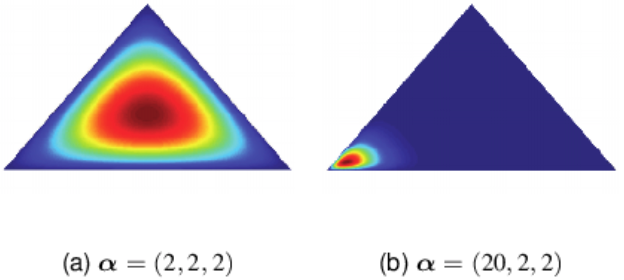
\includegraphics[width=0.8\columnwidth]{images/12b-dirichlet}
	\end{center}
	
\end{itemize}
\subsection{Finite and infinite mixtures}
\subsubsection{Finite Gaussian Mixture Model: } Fixed, finite number of clusters $K$
	\begin{itemize}
		\item Center of cluisters $\mu_k\sim \mathcal N(\mu_0, \sigma_0)$
		\item Prob. of the clusters (parameters) $\rho_{1...K}\sim \mathit{Dir}(\alpha_{1...K})$
		\item Assignments to clusters $z_i\sim \mathit{Categorical}(\rho_{1...K})$
		\item Coordinates of data points $x_i \sim \mathcal N(\mu_{z_i}, \sigma_{z_i})$
	\end{itemize} 
\subsubsection{Selecting $K$: }
\textbf{Issues: }
\begin{itemize}
	\item There might be multiple possible ways to cluster data (hence multiple $K$ that would fit)
\end{itemize}

\textbf{Adaptation: }
\begin{itemize}
	\item Number of clusters might be unknown in advance (movie genres, topics of documents, image segmentation, streaming data, ...)
	\item Naive solution: Select $K$, cluster with EM, evaluate the result and iterate
\end{itemize}

\textbf{What if we just select a large enough $K$? }

\begin{minipage}{\columnwidth}
	\begin{center}
		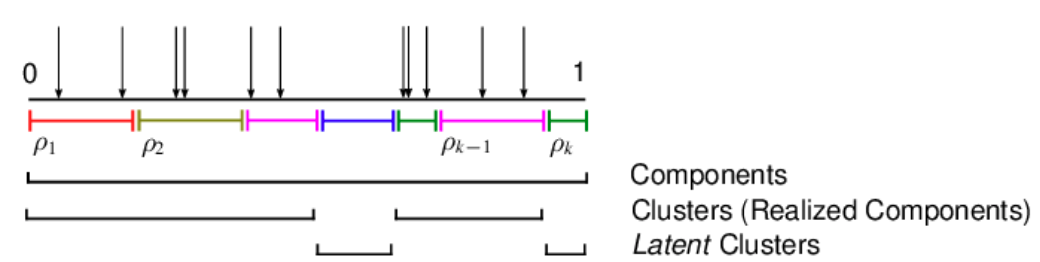
\includegraphics[width=\columnwidth]{images/12b-latent-clusters}
	\end{center}
	\textit{\textbf{Latent clusters: }For a finite number of drawings $N$, we do not have to realize all $K$ clusters. All components will be realized with probability $1$, but only when $N\to\infty$}
\end{minipage}

\begin{itemize}
	\item Select a large $K$, only realize some of them and get more when needed
	\item This only solves the problem partially: How large should this $K$ be? Our belief in $K$ could change as we observe more data-points. We still have issues with streaming/growing data.
	\item \textbf{Solution: Select $k=\infty$}
\end{itemize}

\subsubsection{Infinite mixture models (Selecting $K=\infty$)}
\begin{itemize}
	\item With $K=\infty$, we have nonparametric Bayesian methods (nonparametric means infinitely many parameters) $\to$ we can keep drawing new parameters
	\item Cannot draw infinite points from $\mathit{Dir}$
\end{itemize}




\subsection{Dirichlet Process (DP) and stick breaking}
We can \textbf{sample from a DP using either Stick-Breaking or the Chinese Restaurant Process}

\subsubsection{Dirichlet Proces}
$\DP(\alpha, H)$ is a distribution over probability distributions on a space $\Theta$.
\begin{itemize}
	\item $\alpha\in\R_{>0}$ is a concentration parameter
	\item $H$ is the base measure on $\Theta$ (the space we want to draw parameters from)
	\item A Sample $G\sim\DP(\alpha, H)$ is a function $G:\Theta\to\R_{\geq 0}$ s.t. $\int_\Theta G(\theta)d\theta=1$
\end{itemize}

\begin{minipage}{\columnwidth}
$\DP(\alpha H)$ is characterized by the following property: \textit{For every partition $(T_1, .., T_k)$ of $\Theta$ and $G\sim \DP(\alpha, H)$ we have (for each tuple drawn from multivariate Dirichlet distribution): }

$$
	(G(T_1), ..., G(T_K))\sim \Dir(\alpha H(T_1), ..., \alpha H(T_k))
$$
\end{minipage}

\subsubsection{Stick-Breaking Process}
\textbf{Observation: } sampling $(\rho_1, ..., \rho_K) \sim \Dir(\alpha_1, ..., \alpha_K)$ is equivalent to sampling $\rho_1 \sim \Beta(\alpha_1, ..., \alpha_K)$ and $(\rho_2, ..., \rho_K) \sim \Dir(\alpha_2, ..., \alpha_K)$

\begin{center}
	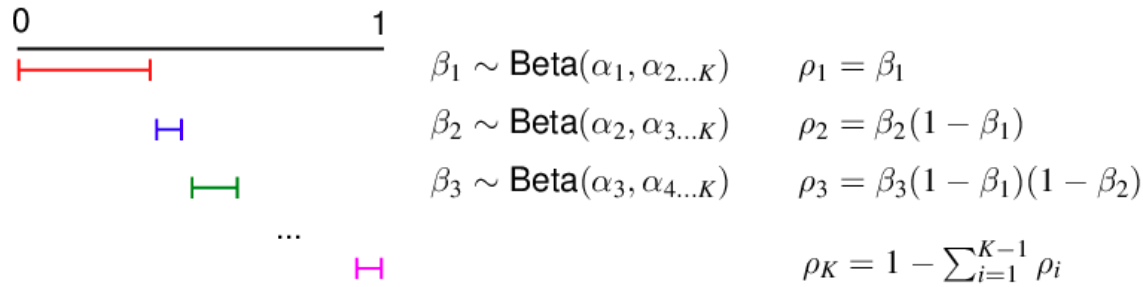
\includegraphics[width = 0.8\columnwidth]{images/12b-stick-breaking-1}
\end{center}
We can keep doing this, but only if $\alpha = (\alpha_1, ..., \alpha_K)$ has finite length $K$.

\textbf{Solution: } fix $\alpha$ s.t. $\beta_i\sim \Beta(1, \alpha) \forall i$
\begin{center}
	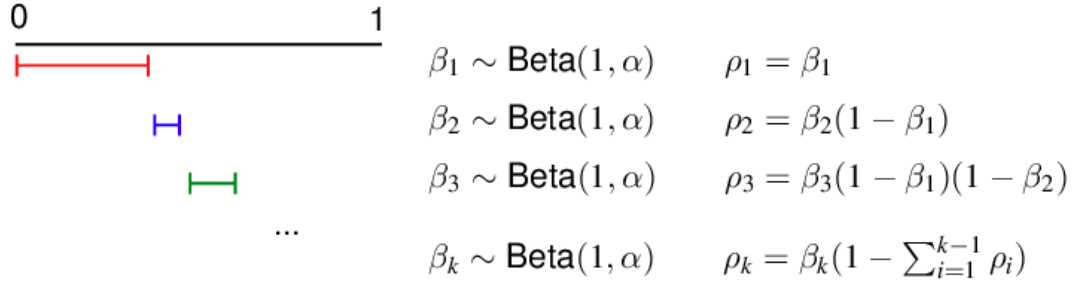
\includegraphics[width =  0.8\columnwidth]{images/12b-stick-breaking-2}
\end{center}

This is called the GEM (Griffiths-Engen-McCloskey) distribution: 
$$
	\rho\sim \GEM (\alpha), \rho.= \{p_k\}_{k = 1}^\infty	
$$

\textbf{Stick-Breaking Construction of the Dirichlet Process: }\\
If $\rho\sim \GEM(\alpha)$ and $\theta_k\sim H$ for $k = 1, 2, ...$, then 
$$
	G(\theta) = \sum_{k=1}^\infty\rho_k\delta_{\theta_k}(\theta)
$$
is a sample from $DP(\alpha, H).$

If we repeatedly sample $\theta^{(1)}, \theta^{(2)}, ...$ from $G\sim \DP(\alpha, H)$, then we have $\theta^{(i)} = \theta_{k_i}$ for some $k_i$.
\begin{itemize}
	\item Sometimes we get a new value $(k_i\neq k_j \forall i<j)$
	\item Sometimes we get a repetition$(k_i =  k_j \text{ for some } i<j)$
	\item Think of $\theta^{(i)}, \theta^{(j)}$ with $k_i = k_j$ as points belonging to the \textbf{same cluster}.
\end{itemize} 

\subsubsection{Chinese Restaurant Process}
\textbf{Technique to draw samples from a Dirichlet Process: }
\begin{itemize}
	\item Join an existing table with probability $\propto$ the number of people already sitting there
	\item Start a new table with probability $\propto \alpha$
\end{itemize}
$$
	P(\textit{customer $n+1$ joins table $\tau$}|\mathcal P) = 
		\begin{cases}
			\frac{|\tau|}{\alpha + n} & \textit{if $\tau \in \mathcal P$} \\
			\frac{\alpha}{\alpha + n} & \textit{Otherwise}
		\end{cases}
$$
\begin{itemize}
	\item $\alpha$ controls the number of new tables ($\alpha$ large: new table likely), 
	\item $|\tau|$ is the number of people on table $\tau$
	\item $\mathcal P$ is a table assignment (partition over the integers)
\end{itemize}


\textbf{Expected number of tables (i.e. clusters) created: }
$$
	\E[\textit{created tables}] = \sumi N\frac{\alpha}{\alpha + i} \sim O(\alpha\log(N)) ]
$$
\textit{"Rich-get-Richer"-effect (preferential attachment): Already popular clusters attract new datapoints}
\subsubsection{Exchangeability}
\textbf{Definition: } Let $(X_1, X_2, ...)$ a sequence of random variables. The sequence is exchangeable when, for every permutation $\pi$ of $\N$. The random vectors
$$
	(X_1, X_2, ...) \quad \textit{ and } \quad (X_{\pi(1)}, X_{\pi(2)}, ...)
$$
have the same distribution.

\textbf{De Finetti's Theorem: } Let $(X_1, X_2, ...)$ be an infinitely exchangeable sequence (one that can be represented by conditionally independent random variables) of random variables. Then $\forall n$
$$
	p(X_1, ..., X_n) = \int \left(\prod_{i = 1}^n p(x_i|G)\right) dP(G)
$$
for some random variable $G$


\textbf{P\'{o}lya Urn}
\begin{itemize}
	\item Urn with colored balls
	\item Draw balls from the urn at random. After drawing a ball, put it back in the urn together with a new ball of the same color
\end{itemize}

\textbf{Hoppe Urn}: P\'{o}lya Urn with special black ball
\begin{itemize}
	\item Urn with colored balls
	\item Draw balls from the urn at random. After drawing 
	\begin{itemize}
		\item If non-black ball: put it back in the urn together with a new ball of the same color
		\item If black ball: put it back in the urn with a new ball of the same color
	\end{itemize}
\end{itemize}

\begin{highlight}{Exchangeability Results}
\begin{itemize}
	\item CRP is identical to the hoppe earn process (we just need to add colors to the tables)
	\item Hoppe Urn and CRP are exchangeable: Can apply \textbf{De Finetti's theorem}
	\item DP is the rancom variable $G$ in De Finetti's theorem for Hoppe urn / CPR
	\item If the prior of $G$ is the DP, then CRP is how we assign points to clusters when we integrate out $G$.
\end{itemize}
\end{highlight}
\subsection{The DP Mixture Model}
$\Theta$ is a set that parametrizes a set of probability distributions, $H$ fixed base measure on $\Theta$. Example:
\begin{itemize}
	\item $\Theta = \R$ with $\mu\in \Theta$ corresponding to $\mathcal N(\mu, \sigma)$ for some fixed $\sigma > 0$
	\item $H = \mathcal N(\mu_0, \sigma_0)$ for some $\mu_0\in \R, \sigma_0\in \R$
\end{itemize}

Based on that we define the \textbf{DP Mixture Model} (a generative model):
\begin{itemize}
	\item Probabilities of clusters ("mixture weights"): $\rho = (\rho_1, \rho_2, ...)\sim\GEM(\alpha)$
	\item Center of clusters $\mu_k\sim \mathcal N(\mu_0, \sigma_0)$
	\item Assignments to clusters $z_i\sim \mathit{Categorical}(\rho)$
	\item Coordinates of data points $x_i \sim \mathcal N(\mu_{z_i}, \sigma)$
\end{itemize}

\subsection{Gibbs sampling}
Useful way of simulating from distributions that are difficult to simulate from directly.

Technique to fit the DPMM (EM considered difficult for nonparametric distributions) by sampling each variable in turn (conditioned on the values of all other variables in the distribution). \textbf{Requires exchangeability}.
\subsubsection{Fitting}
Leverage exchangeability: Any point can be considered "last arrived". Change the assignment of te element without influencing other assignments.
\begin{itemize}
	\item \textbf{Prior}: Probabilities of table assignments w.r.t people seating (cluster size)
	\item \textbf{Posterior}: Probability of the point given the cluster centers
\end{itemize}

\subsubsection{Gibbs Sampling for Fitting}
\begin{minipage}{\columnwidth}
\textbf{Probability Distribution: Collapsed Gibbs sampling formulation}
\begin{align*}
	&p(z_i=k|\z_{-i},\x,\alpha,\mu) \\	
		&\propto p(z_i=k|\z_{-i},\alpha,\cancel{\mu})p(\x|z_i=k,\z_{-i},\cancel\alpha,\mu) \\
		&\propto p(z_i=k|\z_{-i},\alpha)p(x_i|\x_{-i},z_i=k, \z_{-i},\mu)p(\x_{-i}|\z_{-i}, \mu) \\
		&\propto 	\underbrace{p(z_i=k|\z_{-i},\alpha)}_{\textit{Prior}}
					\underbrace{p(x_i|\x_{-i},z_i=k, \z_{-i},\mu)}_{\textit{Likelihood}}
\end{align*}
where $\z_{i}$ and  $\x_{i}$ are the assignments and points excluding the considered point $i$.
\end{minipage}

\textbf{Prior: }
$$
	p(z_i=k|\z_{-i},\alpha) = 
		\begin{cases}
			\frac{N_{k, -i}}{\alpha + N - 1} 	& \textit{For existing $k$} \\
			\frac{\alpha}{\alpha + N - 1} 		& \textit{otherwise} 
		\end{cases}
$$
where $N_{k, -i}$ is the number of elements sitting at table $k$ excluding $i$ $(|\tau\backslash i|)$

\textbf{Posterior: } Observe that if $z_i = k$ we don't need to consider points in $\x$ that are not in $k$. \\
Let $\x_{-i, c} = \{x_j:z_j=c, j\neq i\}$ the data assignment to cluster $c$, then

\begin{multline*}
	p(x_i|\x_{-i},z_i=k, \z_{-i},\mu) = \\
		\begin{cases}
			p(x_i| \x_{-i, k}, \mu) = \frac{p(x_i, \x_{-i, k}|\mu)}{p(\x_{-i, k}|\mu)} & \textit{for existing $k$} \\
			p(x_i|\mu) & \textit{otherwise}
		\end{cases}
\end{multline*}

\subsubsection{Final Collapsed Gibbs sampler: }
\begin{multline*}
	p(z_i=k|\z_{-i},\x,\alpha,\mu) = \textit{Prior} \times \textit{Likelihood} \\
	= \begin{cases}
			\frac{N_{k, -i}}{\alpha + N - 1} p(x_i| \x_{-i, k}, \mu)	& \textit{For existing $k$} \\
			\frac{\alpha}{\alpha + N - 1} p(x_i|\mu)		& \textit{otherwise} 
		\end{cases}
\end{multline*}
	
\begin{algorithm}[H]  
	\For{$i = 1$ to $N$ in random order}{
		Remove $x_i$'s sufficient statistics from old cluster $z_i$ \\
		\For{$k = 1$ to $K$}{
			Compute $p_k(x_i) = p_k(x_i|\x_{-i, k})$ \\
			Set $N_{k, -i} = |\x{-i, k}|$	\\
			Compute $p(z_i=k|\z_{-i},\x) = \frac{N_{k, -i}}{\alpha + N-1}p_k(x_i)$
		}
		Compute $p_*(x_i) = p(x_i|\mu)$ 		\textit{(new cluster)}\\
		Compute $p(z_i=*|\z_{-i}, \x)$ \\
		Normalize $p(z_i|\cdot)$ \\
		Sample $z_i\sim p(z_i|\cdot)$\\
		Add $x_i$'s sufficient statistics to new cluster $z_i$ \\
		If any cluster is empty, rmeove it and decrease $K$\\
	}
	\caption{Collapsed Gibbs sampler for DP mixtures}
\end{algorithm}

\subsubsection{Latent Dirichlet Allocation}
\begin{itemize}
	\item Popular nonparametric Bayesian method
	\item Extension of the model we just defined
	\item \textbf{support multivariate distributions} (e.g. topic modeling on documents, each document belongs to more than one topic; mixture over topics $\to$ multivariate)
\end{itemize}

Given $K$ topics and $V$ words in the vocabulary, for $M$ documents with $N$ words each:\\

\begin{minipage}{0.5\columnwidth}
Distribution of topics in doc. $d$: 
$$
	\theta_d\sim\Dir(\alpha)
$$

Topic that word $w$ in $d$ belongs to:
$$
	z_{d,w} \sim \mathit{Categorical}(\theta_d)
$$

Distribution of words in topic $k$:
$$
	\varphi_k \sim \Dir(\beta)
$$

word $w$ in document $d$: 
$$
	w_{d,w}\sim \mathit{Categorical}(\varphi_{z_{d,w}})
$$
\end{minipage}
\begin{minipage}{0.4\columnwidth}
	\begin{center}
		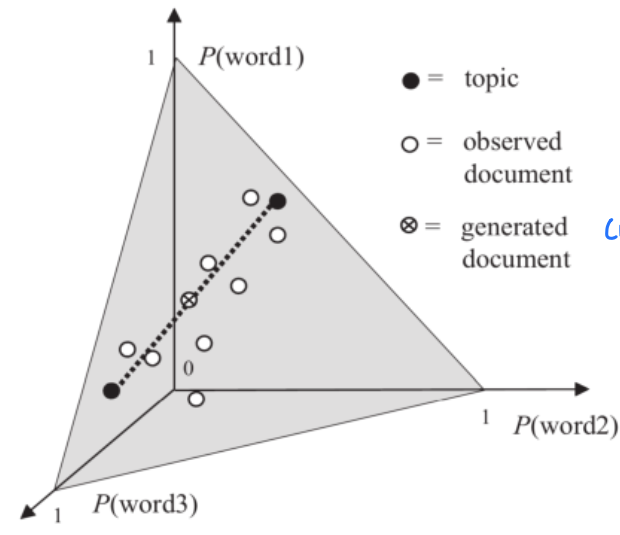
\includegraphics[width=\columnwidth]{images/12b-lda}
	\end{center}
	$\alpha$ controls prior weights of topics in documents, $\beta$ controls prior weights of words in topic
\end{minipage}



